%==============================================================================
% Sjabloon poster bachproef
%==============================================================================
% Gebaseerd op document class `a0poster' door Gerlinde Kettl en Matthias Weiser
% Aangepast voor gebruik aan HOGENT door Jens Buysse en Bert Van Vreckem

\documentclass[english,a0,portrait]{hogent-poster}

% Info over de opleiding
\course{Thesis}
\studyprogramme{Applied Information Technology}
\academicyear{2024-2025}
\institution{University of Applied Sciences and Arts Ghent, Valentin Vaerwyckweg 1, 9000 Ghent, Belgium}

% Info over de bachelorproef
\title{AI jury-assistent voor het herkennen van rope skipping skills in videos.}
% \subtitle{Ondertitel (eventueel)}
\author{Mike De Decker}
\email{mike.dedecker@student.hogent.be}
\supervisor{Ms. L. De Mol \& Mr. T. Parmentier}
\cosupervisor{Mr. D. Plummer (Case Western Reserve University / NextJump)}

% Indien ingevuld, wordt deze informatie toegevoegd aan het einde van de
% abstract. Zet in commentaar als je dit niet wilt.
\specialisation{AI- \& Data Engnineer}
\keywords{Computer vision, Machine Learning, Neural networks, Human Activity Recognition, video classification, YOLO, YOLOv11, MViT, Multiscale Vision Transformer, Swin Transformer, Jump Rope, Rope Skipping, judging, sport}
\projectrepo{https://github.com/mikeddecker/judge}

\begin{document}

\maketitle

\begin{abstract}
Judging the difficulty of jump rope freestyles at high competitve levels, is prone to human errors. It is hard to calculate the correct skill level performed by multiple athles, each performing an action, skill modifier or rope manipulation.
Even though a routine consists of forty to sixty skills, wrongly assigning a single level may impact the ranking, deciding which team is allowed to perform on national or international competitions. In order to correctly assign levels, difficulty judges at higher level competitions are allowed to review the routine at slower speeds in order to increase the accuracy of assigned scores.
This is why this research looked for a way to recognize skills in a video. The scope has been limited to recognizing double dutch single freestyles. The solution provided in this research includes a sequential execution of three steps. The first step involves localizing the athletes in order to crop them out of the video. This cropped video can be used in the second step, namely segmenting the video into individual skill sections. Finally, each individual skill section can then be fed into the recognition model, predicting all aspects of the skills performed by the athletes. Training on a skewed limited dataset of less than an hour, containing about 2500 skills, show that more occuring skills reach an accuracy between 80-99\%, while the lesser occuring skills reach a limited accuracy or even none at all. Mapping the skill predictions to scores, and comparing it to judges, reaches a minus 20.94\% score difference as compared to the score assigned by judges. Populating the (train and test) dataset with more examples, should greatly increase the accuracy. Not only is this interesting for jump rope, but for other sports or movement analysis in general.

\end{abstract}

\begin{multicols}{2} % This is how many columns your poster will be broken into, a portrait poster is generally split into 2 columns

\section{Introductie}

Be quiet! Found them? In Mercia?! The coconut's tropical! But you are dressed as one… Well, what do you want? Knights of Ni, we are but simple travelers who seek the enchanter who lives beyond these woods.

Well, what do you want? It's only a model. Camelot! We found them. We shall say `Ni' again to you, if you do not appease us.

The nose? Shut up! Burn her! I am your king. You don't vote for kings.

You can't expect to wield supreme power just `cause some watery tart threw a sword at you! Well, we did do the nose. I don't want to talk to you no more, you empty-headed animal food trough water! I fart in your general direction! Your mother was a hamster and your father smelt of elderberries! Now leave before I am forced to taunt you a second time!

Why do you think that she is a witch? We want a shrubbery!! I don't want to talk to you no more, you empty-headed animal food trough water! I fart in your general direction! Your mother was a hamster and your father smelt of elderberries! Now leave before I am forced to taunt you a second time!

\section{Experimenten}

A newt? Camelot! Why? No, no, no! Yes, yes. A bit. But she's got a wart.

Shut up! I dunno. Must be a king. Who's that then? Look, my liege! On second thoughts, let's not go there. It is a silly place.

Shut up! Will you shut up?! No, no, no! Yes, yes. A bit. But she's got a wart. He hasn't got shit all over him. It's only a model. It's only a model.

Bring her forward! I don't want to talk to you no more, you empty-headed animal food trough water! I fart in your general direction! Your mother was a hamster and your father smelt of elderberries! Now leave 

\section{Sectie met figuur}

De {\LaTeX} figure-omgeving bepaalt zelf waar een afbeelding komt en dat is meestal niet op de plek in de tekst waar de figure-omgeving gedefinieerd wordt. Als je wilt forceren dat afbeeldingen toch in de flow van de tekst blijven, dan kan je dat zoals hieronder:

\begin{center}
  \captionsetup{type=figure}
  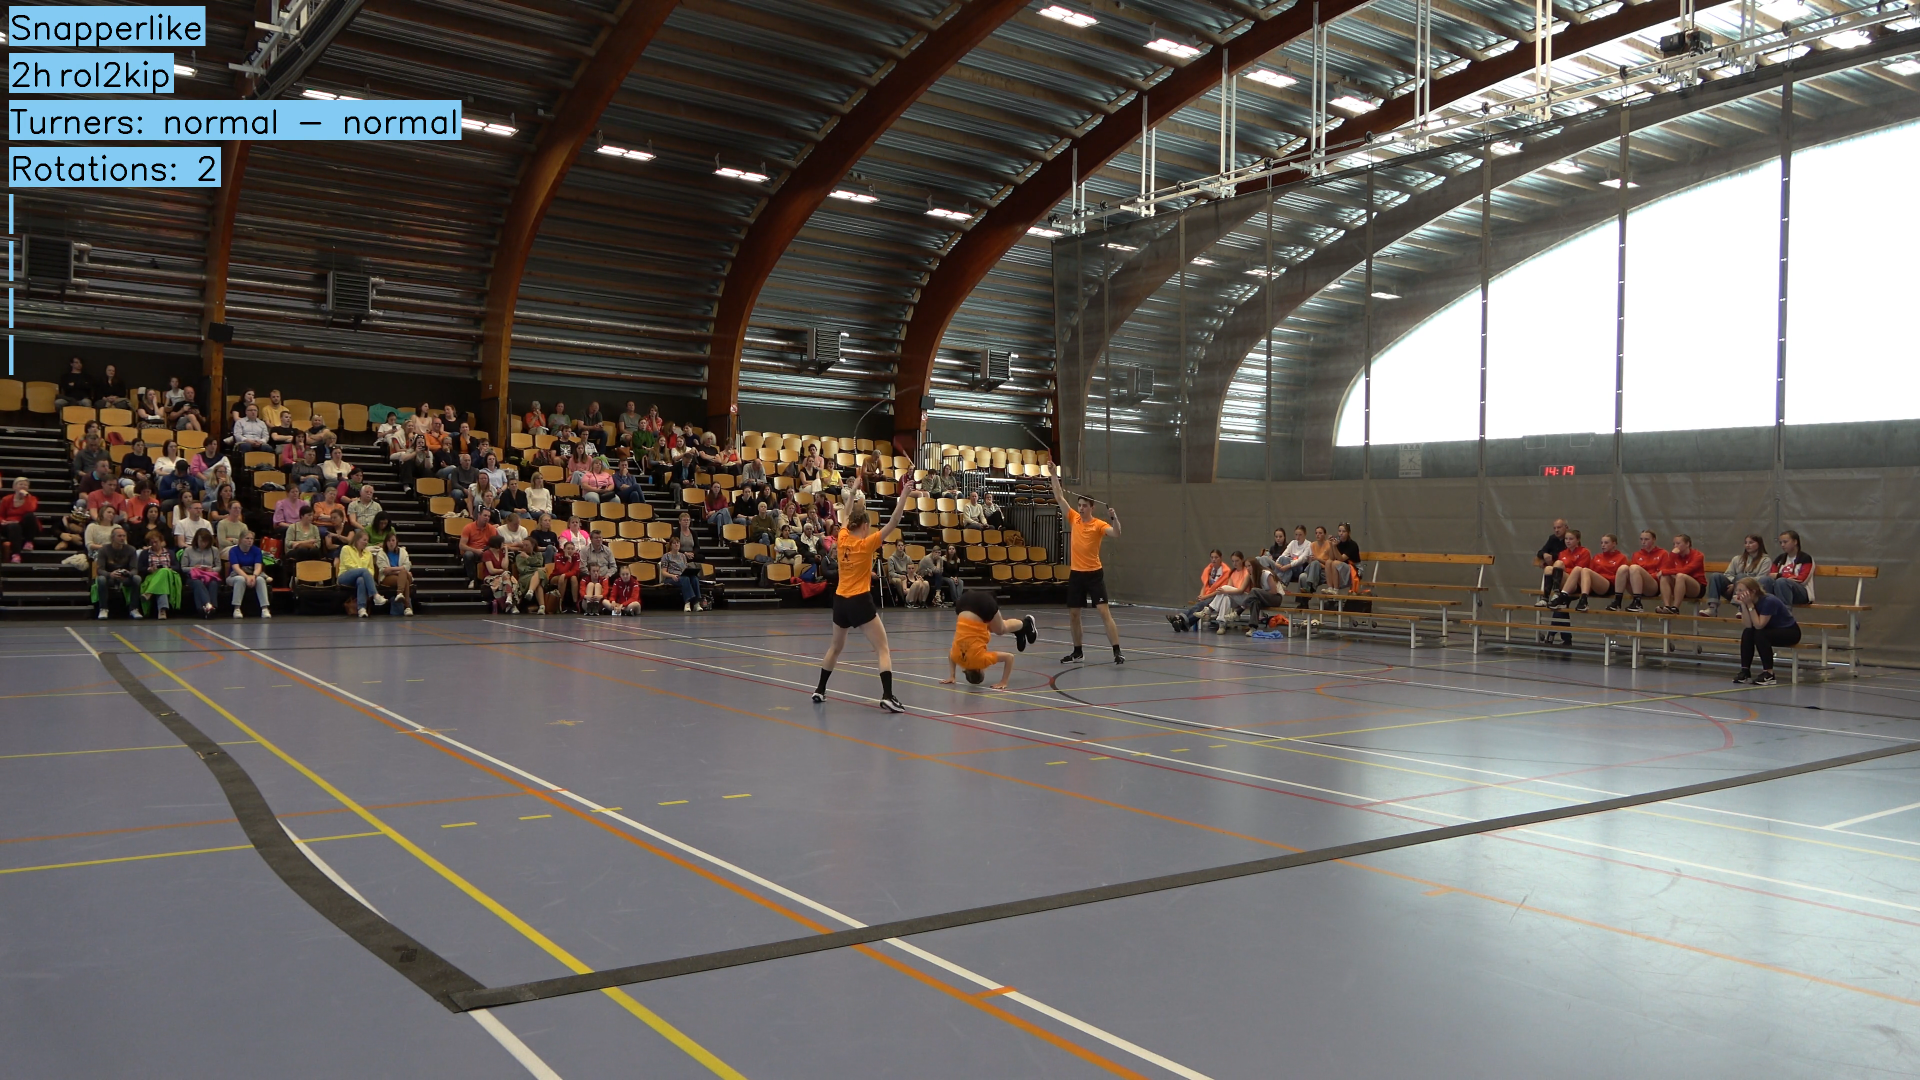
\includegraphics[width=1.0\linewidth]{dd3-example}
  \captionof{figure}{Prediction example displayed as text on a full double dutch singe freestyle video.}
\end{center}

Let er wel op dat dit tot problemen met bladschikking kan leiden.

\section{Conclusies}

Don't underestimate the Force. Oh God, my uncle. How am I ever gonna explain this? I suggest you try it again, Luke. This time, let go your conscious self and act on instinct. Don't be too proud of this technological terror you've constructed. The ability to destroy a planet is insignificant next to the power of the Force.

\section{Toekomstig onderzoek}

I care. So, what do you think of her, Han? No! Alderaan is peaceful. We have no weapons. You can't possibly… I have traced the Rebel spies to her. Now she is my only link to finding their secret base.

Kid, I've flown from one side of this galaxy to the other. I've seen a lot of strange stuff, but I've never seen anything to make me believe there's one all-powerful Force controlling everything. There's no mystical energy field that controls my destiny. It's all a lot of simple tricks and nonsense. You are a part of the Rebel Alliance and a traitor! Take her away! 

\end{multicols}
\end{document}